\documentclass[12pt]{article}
\usepackage{geometry}
\geometry{letterpaper, margin=1in}
\setlength{\parskip}{1em}
\setlength{\parindent}{0pt}
\usepackage{hyperref}
\usepackage{enumitem}
\usepackage{url}
\usepackage{tabularx}
\usepackage{longtable}
\usepackage{booktabs}
\usepackage[english]{babel}
\usepackage{dirtytalk}
\usepackage{amsmath, amssymb, amsthm, graphicx, hyperref}
\usepackage{multicol}


\usepackage{tikz}
\usepackage{pgfplots}
\pgfplotsset{compat=1.17}


\title{Interpreting the Density Function of a Continuous Random Variable}
\author{POL201.01}
\date{}

\begin{document}

% Optional: Customize box padding and border thickness
\setlength{\fboxsep}{8pt}   % Padding inside box
\setlength{\fboxrule}{0.5pt} % Thickness of box border

\maketitle

In this short note, we clarify the intuitive interpretation of the PDF or Density function for a continuous random variable.

In the case of a \textbf{continuous random variable} $X$, the \textbf{probability density function (PDF)} $f_X(x)$ does \emph{not} give the probability that $X$ equals a specific value. In fact, for any single point $x$, we always have:
\[
P(X = x) = 0
\]

Instead, the PDF allows us to compute the probability that $X$ falls within an interval:
\[
P(a \leq X \leq b) = \int_a^b f_X(x) \, dx =
\begin{array}{l}
\text{Area under } f_X(x) \text{ and above the $x$-axis} \\
\text{that accumulates between } a \text{ and } b
\end{array}
\]

\fbox{%
\begin{minipage}{0.53\textwidth}
\vspace{2em}
\begin{center}
    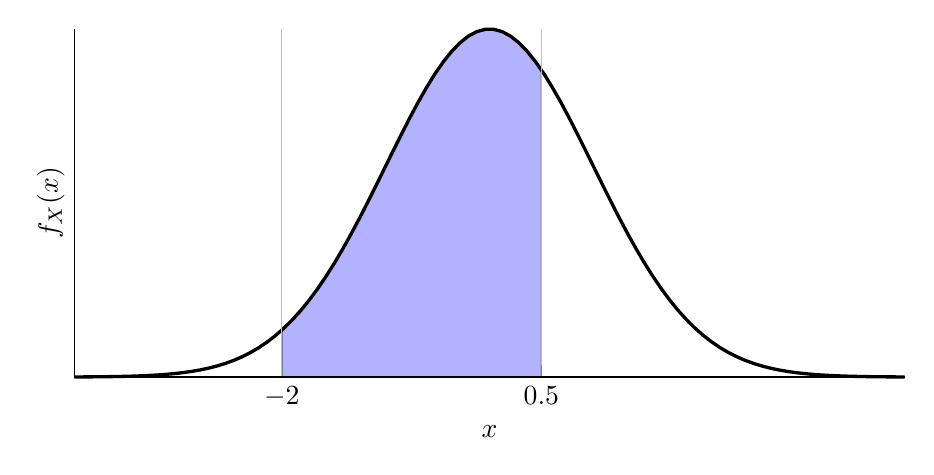
\begin{tikzpicture}
      \begin{axis}[
          no markers,
          domain=-4:4,
          samples=100,
          axis lines*=left,
          xlabel={$x$},
          ylabel={$f_X(x)$},
          height=6cm,
          width=\linewidth,
          xtick={-2,0.5},
          xticklabels={$-2$, $0.5$},
          ytick=\empty,
          enlargelimits=false,
          clip=false,
          axis on top,
          grid = major
        ]

        % Fill area between -2 and 0.5 under the normal curve
        \addplot [
          fill=blue!30,
          domain=-2:0.5
        ]
        {1/sqrt(2*pi)*exp(-x^2/2)} \closedcycle;

        % Draw the standard normal curve
        \addplot [
          very thick,
          domain=-4:4
        ]
        {1/sqrt(2*pi)*exp(-x^2/2)};
      \end{axis}
    \end{tikzpicture}
\end{center}

\end{minipage}
\begin{minipage}{0.43\textwidth}
    This figure shows the probability:
    \[
    P(-2 \leq X \leq 0.5) = \int_{-2}^{0.5} \dfrac{1}{\sqrt{2\pi}}e^{ \frac{-x^2}{2}} \, dx
    \]
    where \( f_X(x) \) is the PDF of the standard normal distribution. The shaded region under the curve between \(-2\) and \(0.5\) represents the total probability mass within that interval.
\end{minipage}
}





\noindent
\textbf{Important Interpretation:} Although $f_X(x)$ is not a probability itself, it can be understood as a \textit{scaled measure of the relative likelihood} of values around $x$. That is, if $f_X(0.5) > f_X(-2)$, then values near $x = 0.5$ are more likely (in a relative sense) than values near $x = -2$.

\begin{itemize}
    \item The term \textbf{scaled} is crucial: $f_X(x)$ is scaled so that the \emph{total area under the curve is 1}, i.e.,
    \[
    \int_{-\infty}^\infty f_X(x) \, dx = 1
    \]
    \item The \emph{shape} of $f_X(x)$ gives insight into which values of $X$ are more or less likely, relatively speaking.
    \item The actual \emph{probability} that $X$ falls in a range is always computed from the \emph{area under the curve} between two points.
\end{itemize}

\bigskip

\noindent
This interpretation is useful for building intuition: the PDF serves as a \textit{relative likelihood landscape}, and the height of the curve at a point $x$ reflects how densely probability is packed near that value.

\bigskip

\noindent
\textbf{Caution:} Do not confuse $f_X(x)$ with the probability that $X = x$. For continuous variables, all point probabilities are zero (i.e., $P(X = x) = 0$)


\end{document}
